\documentclass[12pt,a4j,titlepage]{ltjsarticle}
\usepackage{semi}
\usepackage{here}

% \title{}
% \author{}
% \date{}

\begin{document}
\begin{titlepage}
  \begin{center}
  
    \vspace*{20truept}
    
    {\LARGE 2022年度 卒業論文} 
    
    \vspace*{75truept}
    
    {\Huge Webサイトの最適な広告配置方法と} %論文タイトル

    \vspace{10truept}

    {\Huge テキストによる印象の調査} %論文タイトル 長い場合 改行1

    \vspace{10truept}

    {\Huge } %論文タイトル 改行2

    \vspace{85truept}
    
    {\LARGE 指導教員 須田 宇宙 准教授}
    
    \vspace{60truept}
    
    {\LARGE 千葉工業大学 情報ネットワーク学科}
    
    \vspace{15truept}
    
    {\LARGE 須田研究室}
    
    \vspace{70truept}
    
    {\LARGE 1932135 氏名 村上 航介 } % 氏名は消さない 学生番号 氏名 名前

    \vspace{70truept}
    
  \end{center}
  \begin{flushright}

    {\LARGE 提出日 2023年1月17日}
  
  \end{flushright}
\end{titlepage}

\setcounter{page}{0}\pagenumbering{roman}\pagestyle{plain}
%\setcounter{tocdepth}{3}
% 目次の出力
\tableofcontents
% 表目次
\listoftables
% 図目次
\listoffigures

\clearpage
\setcounter{page}{0}\pagenumbering{arabic}

\section{緒言}
\label{sec:1}
近年,インターネット市場が年々需要が高まっているなか,広告において,TV・新聞などのマスメディアよりも,検索エンジン,Webサイト,アプリ,SNSなど,インターネットを介して利用するメディアやサービスに広告を掲載する企業が増加している.
また,インターネット広告自体のテキストのフォントの色使い,大きさなどの印象により、宣伝効果や煩わしさに影響するのかは明確になっていない.

Webサイトに広告を掲載することに対して,広告をページ上のどこに,どのように配置するかが重要な点であると考える.
広告の配置によっては,ユーザにとって煩わしい位置にあるWebページが存在し,広告収益によるトレードオフを考えながら配置する必要があるが,配置方法によって,ユーザに与える煩わしさや広告の宣伝効果の関係は,はっきりわかっていない.
これに対して,モバイル端末における広告配置についての研究があり,クリック率を優先する場合には,ユーザがスクロールを行った際に,視線の先に広告が表示される配置や視線の逆方向に配置する方法が有力となり,煩わしさの軽減を優先する場合には,Webページ内の特定の部分に表示される方法や常に上部に表示される方法が有力な配置方法として挙げられている\cite{mobile}.
しかし,パソコン上での宣伝効果に適した広告配置が明らかになっていないという問題点があり,また,フォントによる印象についての研究は行われているが,広告におけるフォントに関する研究が行われていないことも問題となっている.

そこで本研究では,パソコン上における,Webサイトにおける広告配置とテキストによる煩わしさおよび宣伝効果の違いや影響を調査し,比較することを目的とする.

\clearpage

\section{インターネット広告}
\subsection{インターネット広告とは}
インターネット広告とは,Webサイトや検索エンジン,SNS,アプリケーションなどに掲載される広告のことを指す.
企業の商品やサービスの広告を各メディア(Webサイト・動画・SNS等)の広告枠に掲載し配信できるシステムとなっており,多くの企業がインターネット広告を利用している.
また,インターネット広告の市場規模において,図\ref{fig:広告費}のように,2021年では,インターネット広告費がマスコミ四媒体広告費用(新聞/雑誌/ラジオ/テレビメディアの媒体費と製作費の合算)を上回ったことが報告されている\cite{dentsu}.

\begin{figure}[h]
\begin{center}
 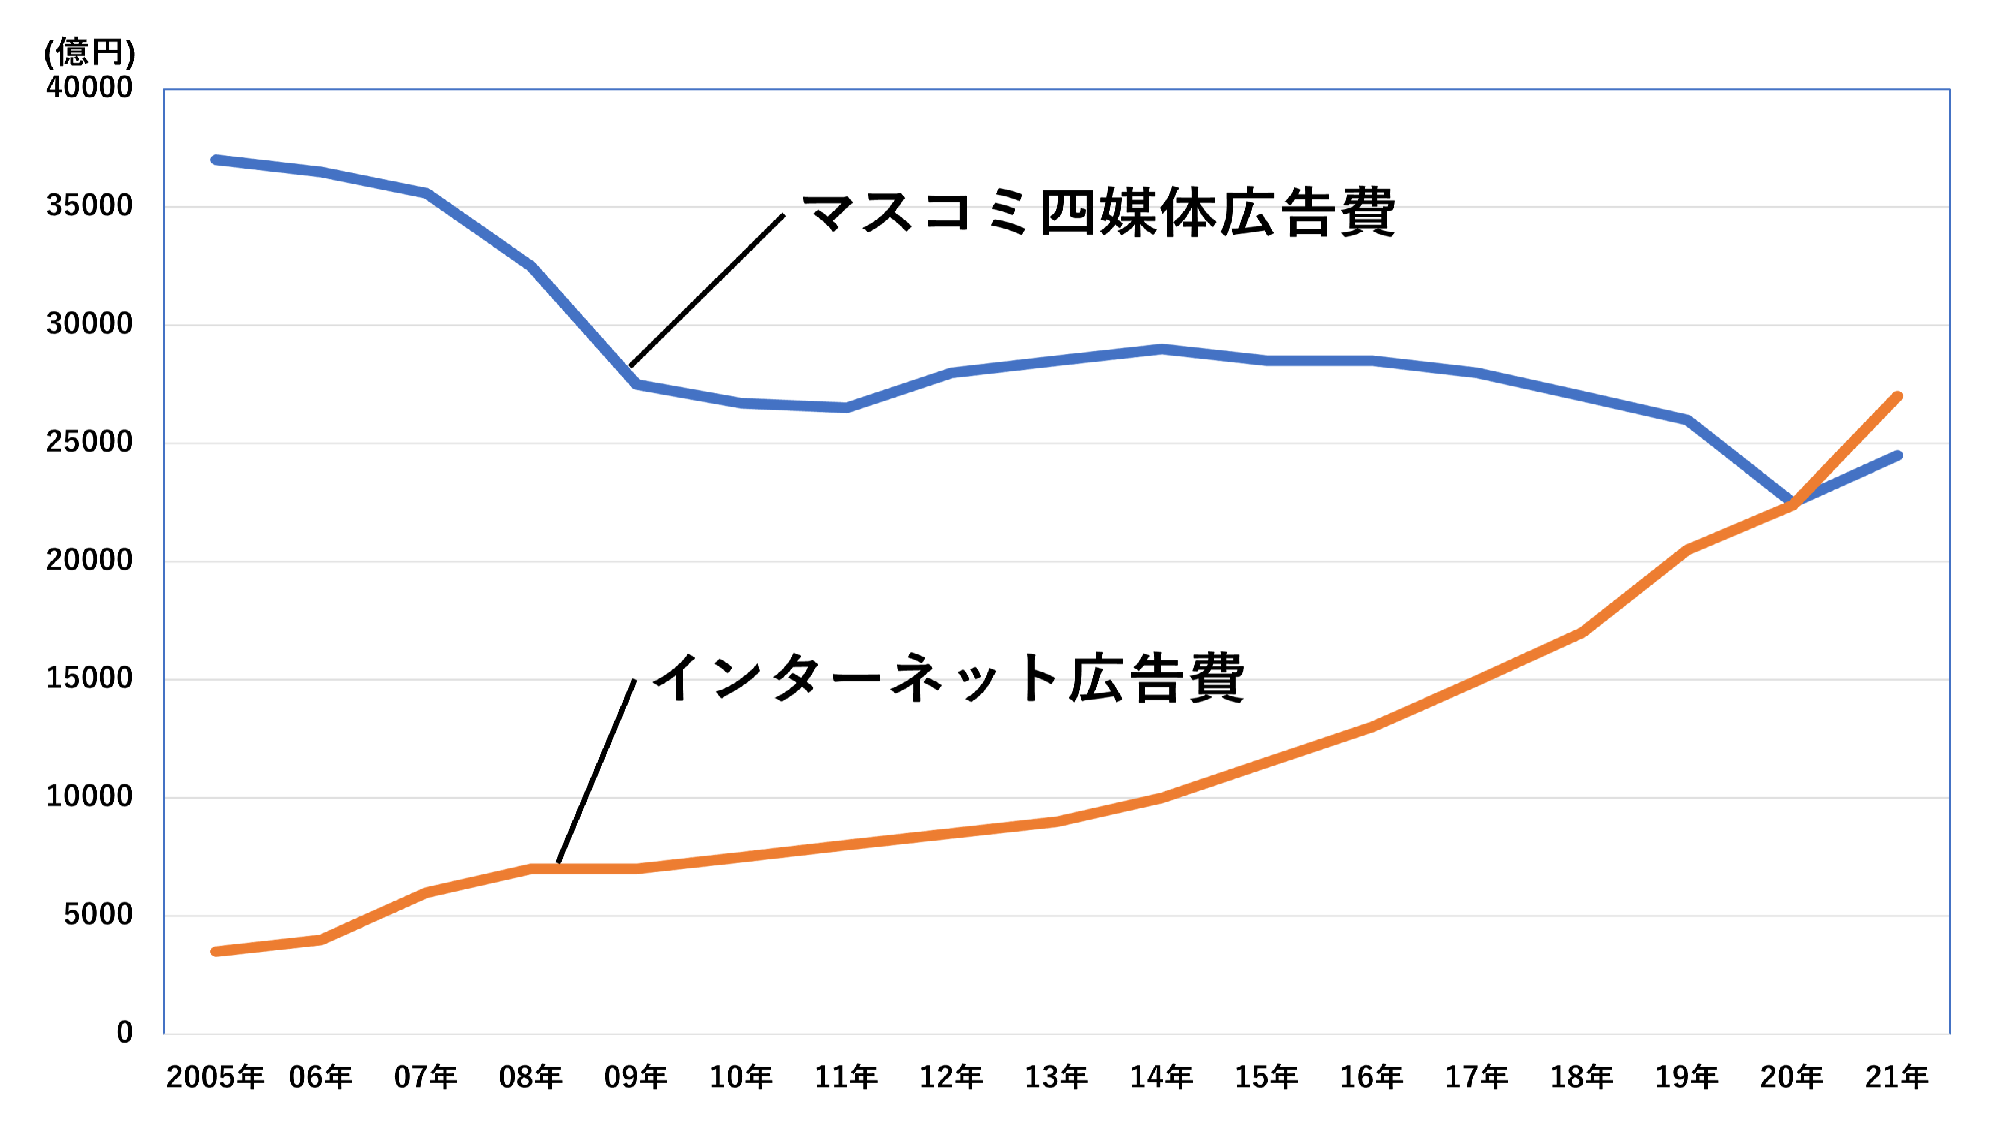
\includegraphics[height=65mm]{広告費.pdf}
\end{center}
 \caption{広告費の推移}
 \label{fig:広告費}
\end{figure}

\subsection{インターネット広告の種類}
\subsubsection{リスティング広告}
\label{subsubsec:rs}
Google・Yahoo!などの検索エンジンで検索をした際に,検索結果画面に表示される広告で,ユーザーが検索したキーワードに連動して検索結果一覧の上部・下部に表示されるので,「検索連動型広告」とも呼ばれる.
Googleなどで検索して一番上にあるサイトにアクセスしようとしたら「広告」と書いてあるそのサイトがリスティング広告である.
そのため,検索キーワードに興味・関心が高い能動的なユーザーに絞って配信できるため,ユーザー自身のニーズが明確になっている顕在層に効果が高い広告と言える.

\subsubsection{ディスプレイ広告}
Webサイトやアプリケーション内の広告枠に表示される画像広告,動画広告,テキスト広告のことで,バナーで表示されることが多いため,「バナー広告」とも呼ばれる.
興味や関心が高いものの自社の商品を知らないユーザーである潜在層にアプローチすることができ,商品やサービスの認知拡大ができる.
また,リスティング広告とは違い,画像や動画を使用できるため,目にとまりやすいというメリットがあり,ビジュアルで表現することで,商品やサービスの魅力をより具体的に伝えることができる.

\subsubsection{SNS広告}
SNS広告とは,Twitter・Facebook・Instagram・LINEなどのSNS上で配信する広告で,タイムラインやストーリーズ,おすすめのアカウント欄に表示される広告などがある.
最大のメリットとしては,ターゲティング精度の高さで、SNSはユーザがアカウントを登録する際に,年齢・性別・役職・趣味など個人情報の登録が求められるので,ユーザデータが蓄積され,それをもとに詳細なターゲティングが可能になる.

\subsubsection{ネイティブ広告}
あるメディアの記事やニュースなどのコンテンツの中に自然と融合している広告で,サイトの中で自然に表示されるので,「広告が挟まっていて不事前」という違和感を与えることなく,ユーザーに情報を届けることができるのが特徴.
また,違和感なくユーザーを誘導して認知してもらう広告手法なので,SNS投稿の一部として表示されるものもあり,Twitterでいうと「プロモーション」がそれに該当する.
ユーザーにストレスを与えることなく誘導でき潜在層にアプローチできるが,コンテンツ作成に労力がかかり,他の広告形態よりも効果を実感できるまでに時間がかかる.

\subsubsection{動画広告}
動画広告とは,その名の通り「動画」を使った広告のことで,静止画の広告よりも一度に多くの情報を伝えることができるので,ユーザの印象に残りやすい傾向にあり,サービスや商品の購入に繋がる可能性が期待できる.
また,効果測定をし,改善することが可能なので,売上増加に繋げることができる.
しかし,YouTubeではスキップされてしまい,SNSに表示される広告では、スクロールされる途中に表示される動画広告もあり,これもYouTube広告同様,興味がなければそのままスクロールされ,視聴されない可能性がある.
そのため,クオリティの高い動画を製作する必要がある.
動画広告の種類としては,YouTubeなどの動画サイトで配信され,動画プレイヤーの大画面の中で再生される「インストリーム広告」や従来のバナー枠に配信されるタイプの「インバナー広告」,ユーザーがWebページをスクロールし,動画広告が画面に表示された瞬間から動画が再生される「インリード広告」が挙げられる.

\subsubsection{オーディオ広告}
\label{subsubsec:ad}
オーディオ(音声)広告とは,音声メディアを通じて配信される広告全般を指しており,従来では,ラジオ放送において番組の合間に流されるCMが音声広告の代表例だったが,Spotifyをはじめとする音楽配信サービスや,radikoをはじめとするインターネットラジオ,各種ポッドキャストなどオンライン上の音声メディアでオーディオ広告が登場している.
耳からの情報伝達であるため,「片手間」のユーザーに情報を届けられ,意識の妨げになりにくいので,視覚的な刺激とは異なる点が多い.

\subsection{スマートフォン広告}
スマートフォン広告は,スマートフォン上でのインターネット広告のことで,スマートフォン上においても\ref{subsubsec:rs}~\ref{subsubsec:ad}での広告形態が存在する.
パソコンとは違い,ちょっとした空き時間に検索する際には感覚的にパッとよさそうなものを閲覧する傾向があるので,スマートフォン広告もこのようなスマートフォンの特性を踏まえなければならない.
掲載方式の種類も様々で,ページの上部・中部・下部に固定して表示されるものやスクロールする方向に追従して表示されるもの,全画面に表示されるものなどが存在する.

\clearpage

\section{先行研究}
\subsection{実験概要}
中島ら(2018)は,「モバイル端末におけるWeb広告の配置方法に対する一検討」というモバイル端末でのインターネット広告の配置方法の比較を行った\cite{mobile}.

本研究の目的は,主な既存の広告配置方法の2つと新たに3つの配置方法の合計5つの広告配置方法を,ユーザに与える煩わしさと宣伝効果の観点から比較することである.
そこで,煩わしさの計測指標としては,被験者が各配置方法に対して行った4段階評価の結果およびコメント文を用いる.
また,宣伝効果の計測指標としては,表示されていた広告の色やロゴ等を正しく認識できていたかを回答する問題の正答率を用いる.
さらに,各広告のクリック率も宣伝効果の指標とする.
本研究では,クラウドソーシングサービスを用いて,インターネット上で250人の被験者を募集し,Webの記事を読むという行為に該当する実験設定で,広告が配置されたメールを10通読んでもらい,メールの内容に関する問題を答えてもらいアンケートを回答する.

\subsection{既存の配置方法}
\begin{enumerate}
\item 静止広告

Webページ内の特定の部分に表示される広告である.
この配置方法ではユーザがスクロールを行うと,広告はページ内の他のコンテンツとともに画面外に流れるため,静止広告はユーザの視界に入りにくいと考えられる.
\item アンカー広告

ユーザがスクロールを行っても画面の下部に表示され続ける広告で,Webのコンテンツは主に上から下に読む構造になっているため,この配置方法では広告がユーザの視界に入りやすいと考えられる.
\end{enumerate}

\subsection{提案する配置方法}
\begin{enumerate}[i]
\item アッパー広告

アンカー広告の逆で,ユーザがスクロールを行っても画面の上部に表示され続ける広告である.
\item フォワード広告

画面の上部または下部に表示され,ユーザがスクロールを行った際に,スクロール先に移動して表示される広告である.
これはユーザがスクロールを行った際に,視線の先に広告が表示されることを意図した配置方法である.

\item バックワード広告

フォワード広告の逆で,ユーザがスクロールを行った際に,スクロール先の逆方向に移動して表示される広告である.
これはユーザがスクロールを行った際に,視線の先から広告が離れることを意図した配置方法である.
\end{enumerate}

\subsection{結果と考察}
\subsubsection{広告の認識正答率}
認識正答率はアンカー広告が23.4\%と最も高く,次いでフォワード広告とバックワード広告が20\%前後で近い値となった.
また,静止広告とアッパー広告はどちらも10\%未満で近い値となった.

\subsubsection{広告の煩わしさ}
静止広告とアッパー広告については,煩わしさを4(最も煩わしい値が4)と評価する被験者は存在せず,煩わしいと評価した被験者の割合はほぼ同じだった.
また,広告を煩わしいと評価した被験者(3または4と評価した被験者)の割合は,フォワード広告とバックワード広告が他の配置方法よりも高かった.

\subsubsection{広告のクリック率}
各広告のクリック率はいずれも 1\%未満という結果になった.
また,アンカー広告をクリックした被験者は存在せず,その他の広告についてもクリック回数は2~3回であった.

\subsubsection{広告に対するコメント文}
煩わしいと記述される割合が最も高いのはバックワード広告であり,煩わしくないと記述される割合が最も高いのは静止広告であることが分かった.

\subsubsection{考察}
\begin{figure}[h]
\begin{center}
 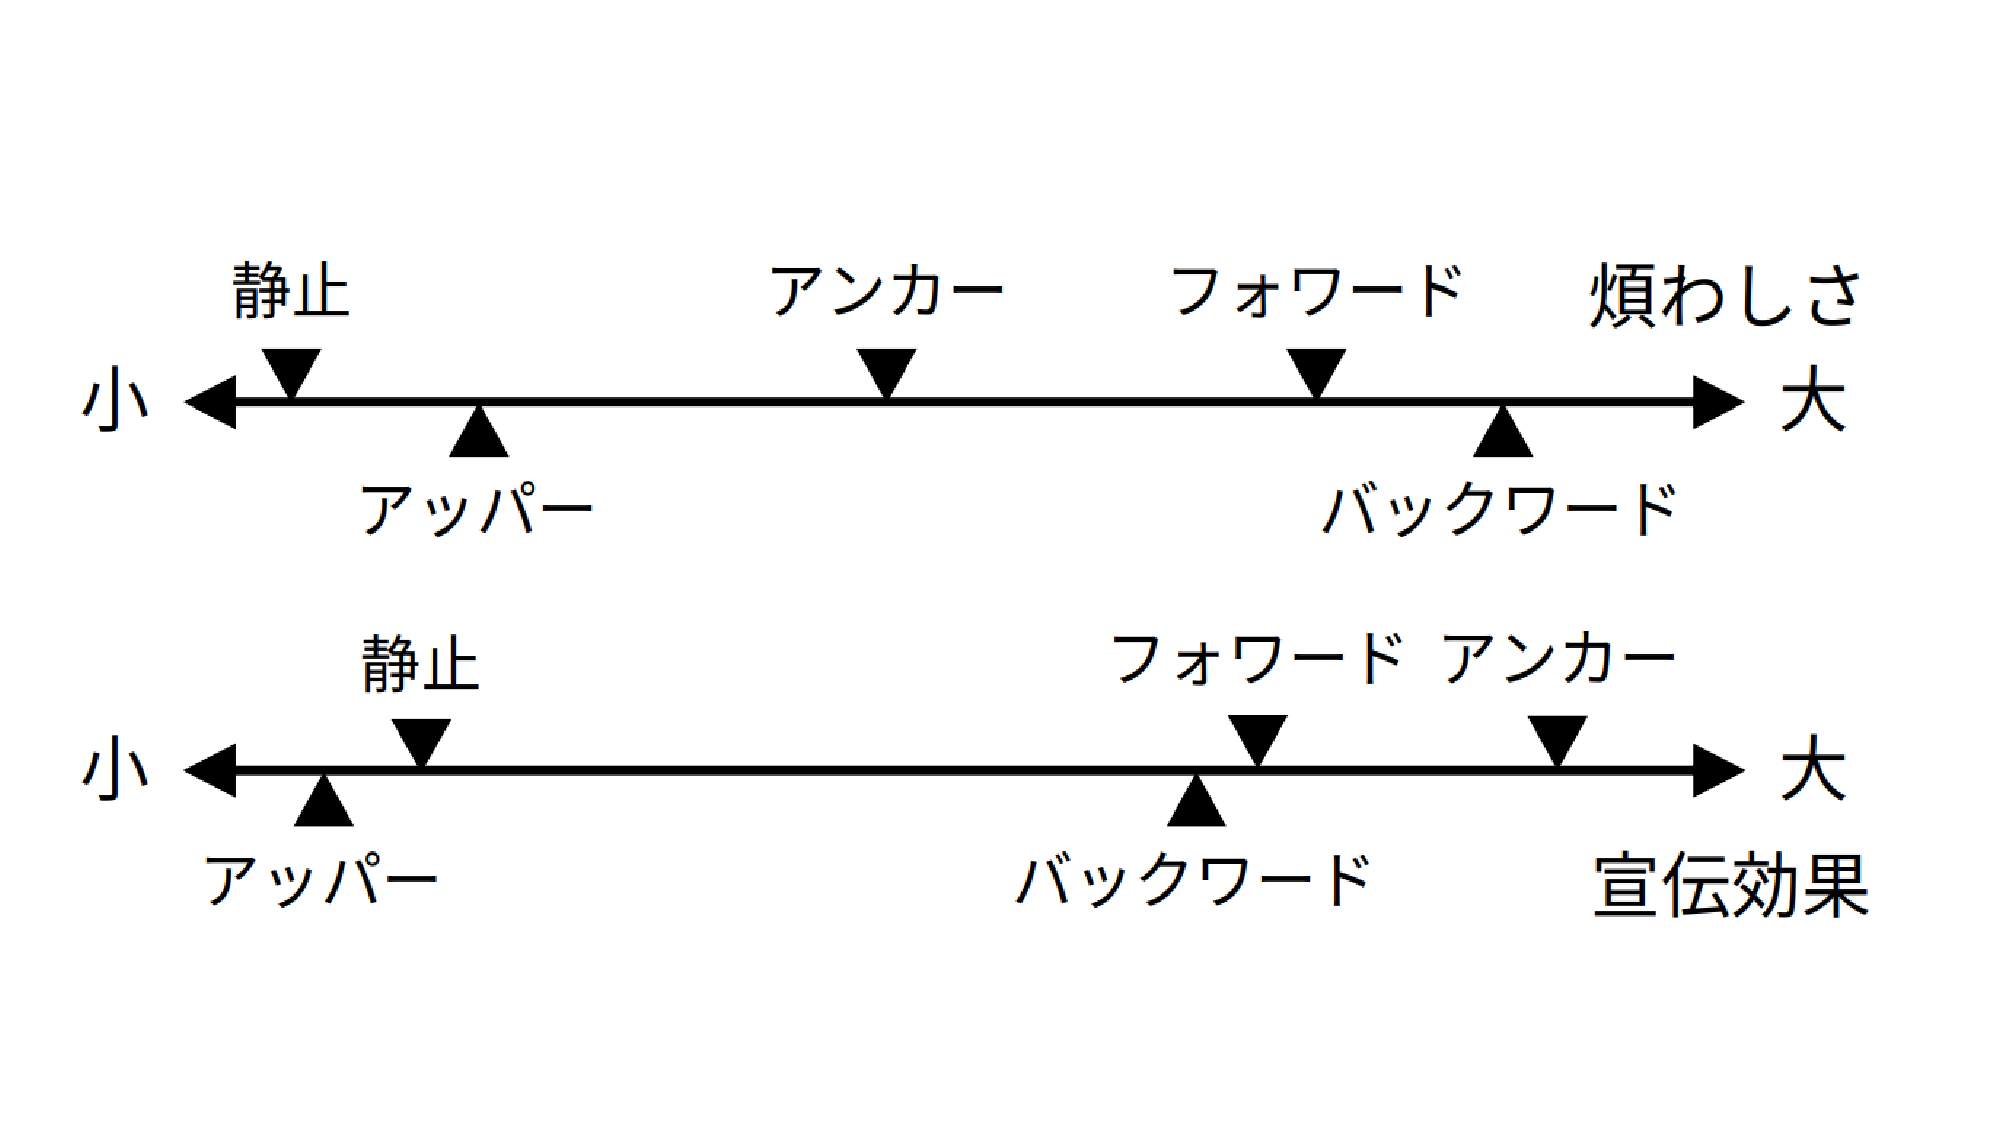
\includegraphics[height=65mm]{figures/先行研究結果.pdf}
\end{center}
 \caption{先行研究の実験結果}
 \label{fig:先行研究結果}
\end{figure}

図\ref{fig:先行研究結果}に配置方法による広告の煩わしさおよび宣伝効果の実験結果を示す.
コンテンツ提供者が広告をどこに,どのように配置するかを考える際の基準について,以下が挙げられる.

\begin{itemize}
\item クリック率を優先する場合

広告収入を最大化するためにクリック率を優先する場合は,フォワード広告やバックワード広告が有力である.

\item 煩わしさの軽減を優先する場合

広告の煩わしさを軽減してユーザ離れを可能な限り減らすことを優先する場合は,静止広告やアッパー広告が有力である.
\end{itemize}

また,広告が認識されることを優先する場合はアンカー広告やフォワード広告,バックワード広告が有力であるが,広告を提供する企業にとって広告が認識されることは重要ではなく,クリックされるかどうかが重要であるため,アンカー広告の優先度は高くないと考えられる.

\clearpage

\section{評価実験}
\subsection{実験概要}
本研究では,パソコン上における,Webサイトの広告配置とテキストによる煩わしさおよび宣伝効果の違いを比較していくため,パソコン上で見ることを前提とする.
テキストのフォントのパターンを調査する目的としては,テキストのフォントの違いで,広告の煩わしさおよび宣伝効果に影響するのかを知るためである.
宣伝効果の指標として,表示されていた広告を正しく認識していたかどうかを回答する問題の正答率を用いる.
煩わしさの指標としては,煩わしさについて4段階評価をしてもらい算出する.
配置のパターンとしては,記事内・記事右部・記事終わりの3パターンで,各パターンで一つずつ記事に配置して,記事を見た後にアンケートを答えてもらう.
テキストのフォントでは,ゴシック体・明朝体・丸ゴシック体の3パターンで,各パターンで一つずつ記事の広告として配置して,記事を見た後にアンケートに答えてもらう.
そのため,広告の配置とテキストのフォントによるパターンを分けて比較していくため,Google Formsを利用して2回アンケートを行う.

また,記事の内容は私の趣味に関するもので,理由としては,趣味に関するものであれば記事を書きやすためである.
また,パソコンで見てもらうのを前提としているので,調査対象は,パソコンを使用することが多い大学生(千葉工業大学の学生)を対象とし,期間として1回目のアンケートでは,10月17日の週から次の週にかけて,2回目のアンケートでは,12月5日の週から次の週にかけて回答を募集した.

\subsection{Web記事の構成}
配置においては,図\ref{fig:記事内}~図\ref{fig:記事終わり}のように記事内・記事右部・記事終わりを示している.
3つのパターンにした理由としては,「Yahoo!ニュース」や「朝日新聞デジタル」などの大手ニュースサイトでは,画面内・記事右部・記事終わりなどに広告が配置されていることが見受けられるので,これらのパターンを中心に比較していく.

\begin{figure}[H]
\begin{center}
 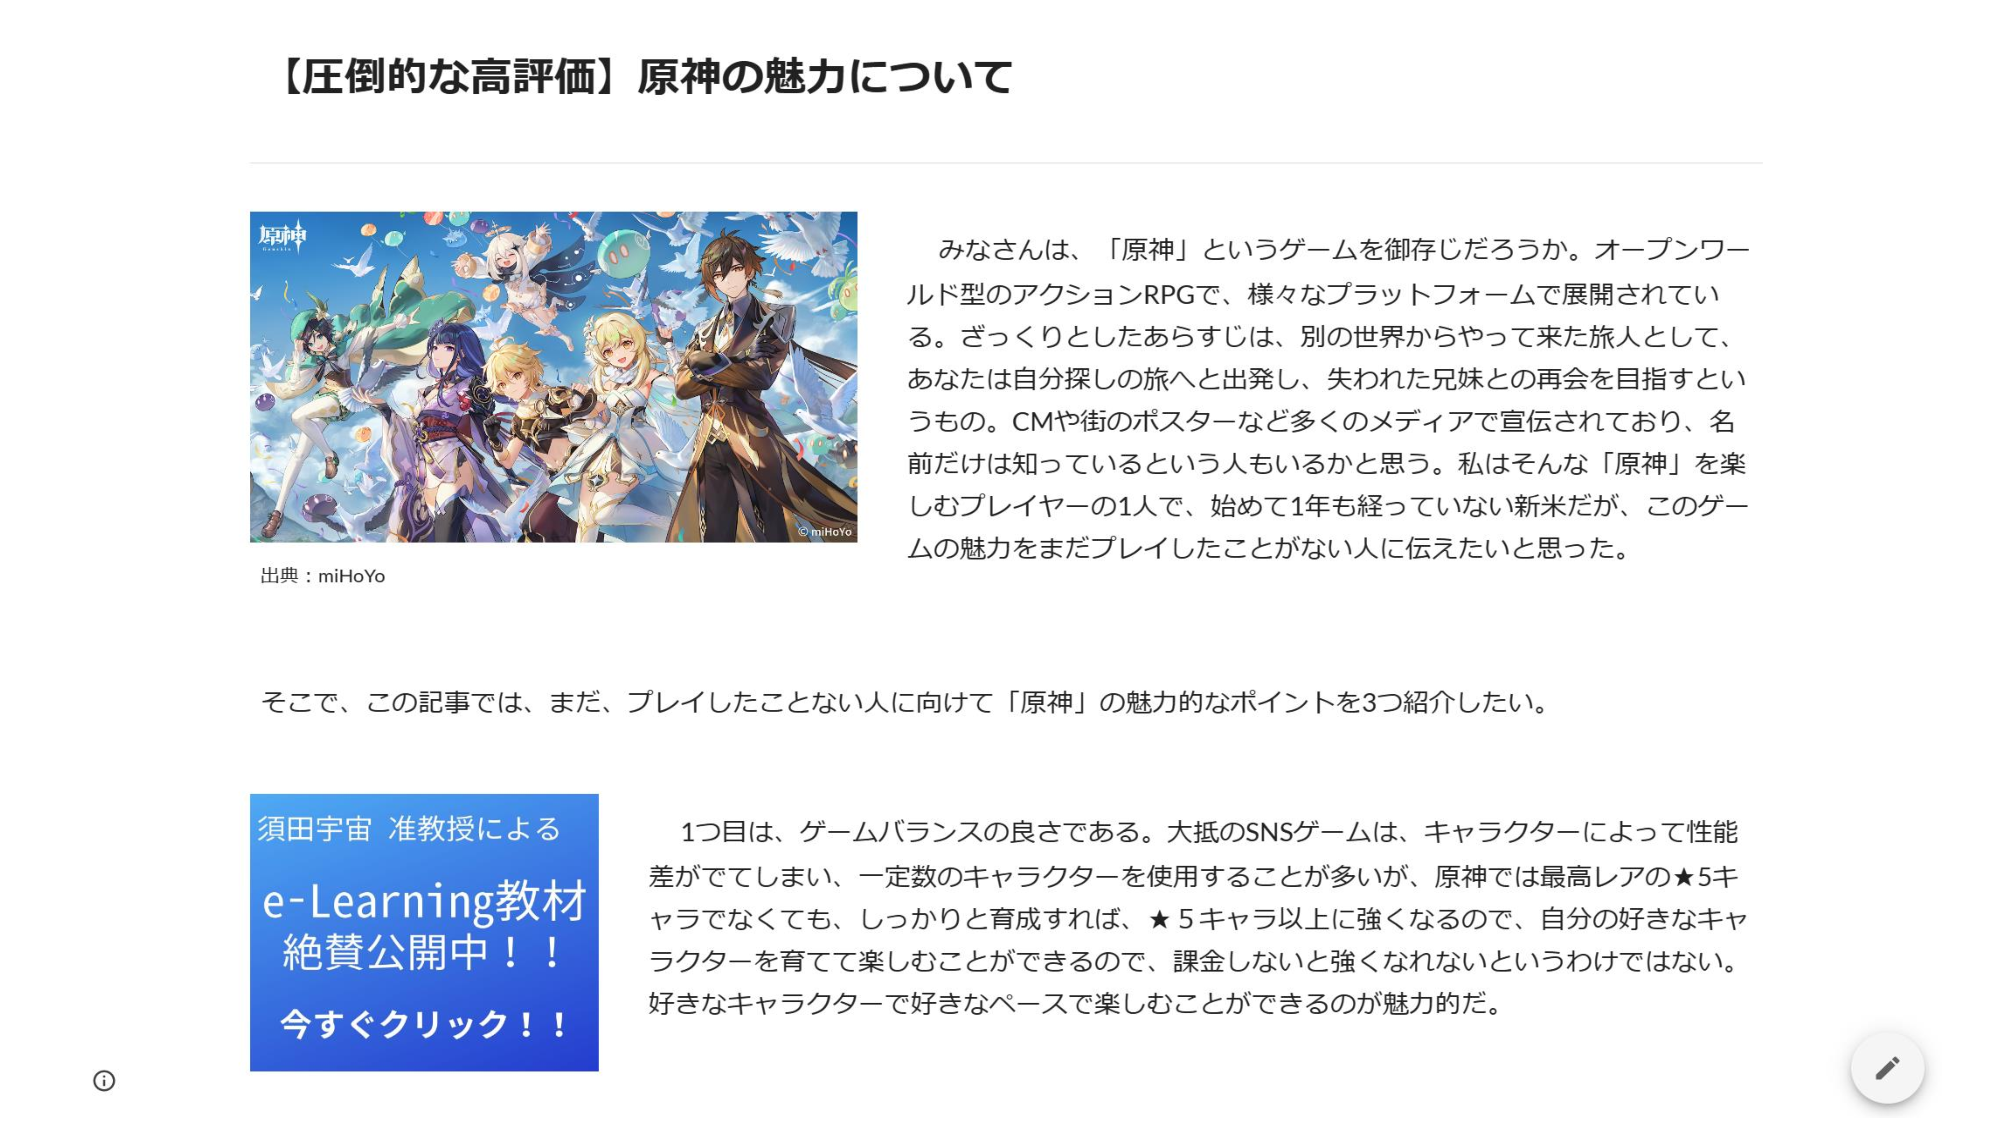
\includegraphics[height=70mm]{figures/記事内.pdf}
\end{center}
 \caption{記事内の配置}
 \label{fig:記事内}
\end{figure}

\begin{figure}[H]
\begin{center}
 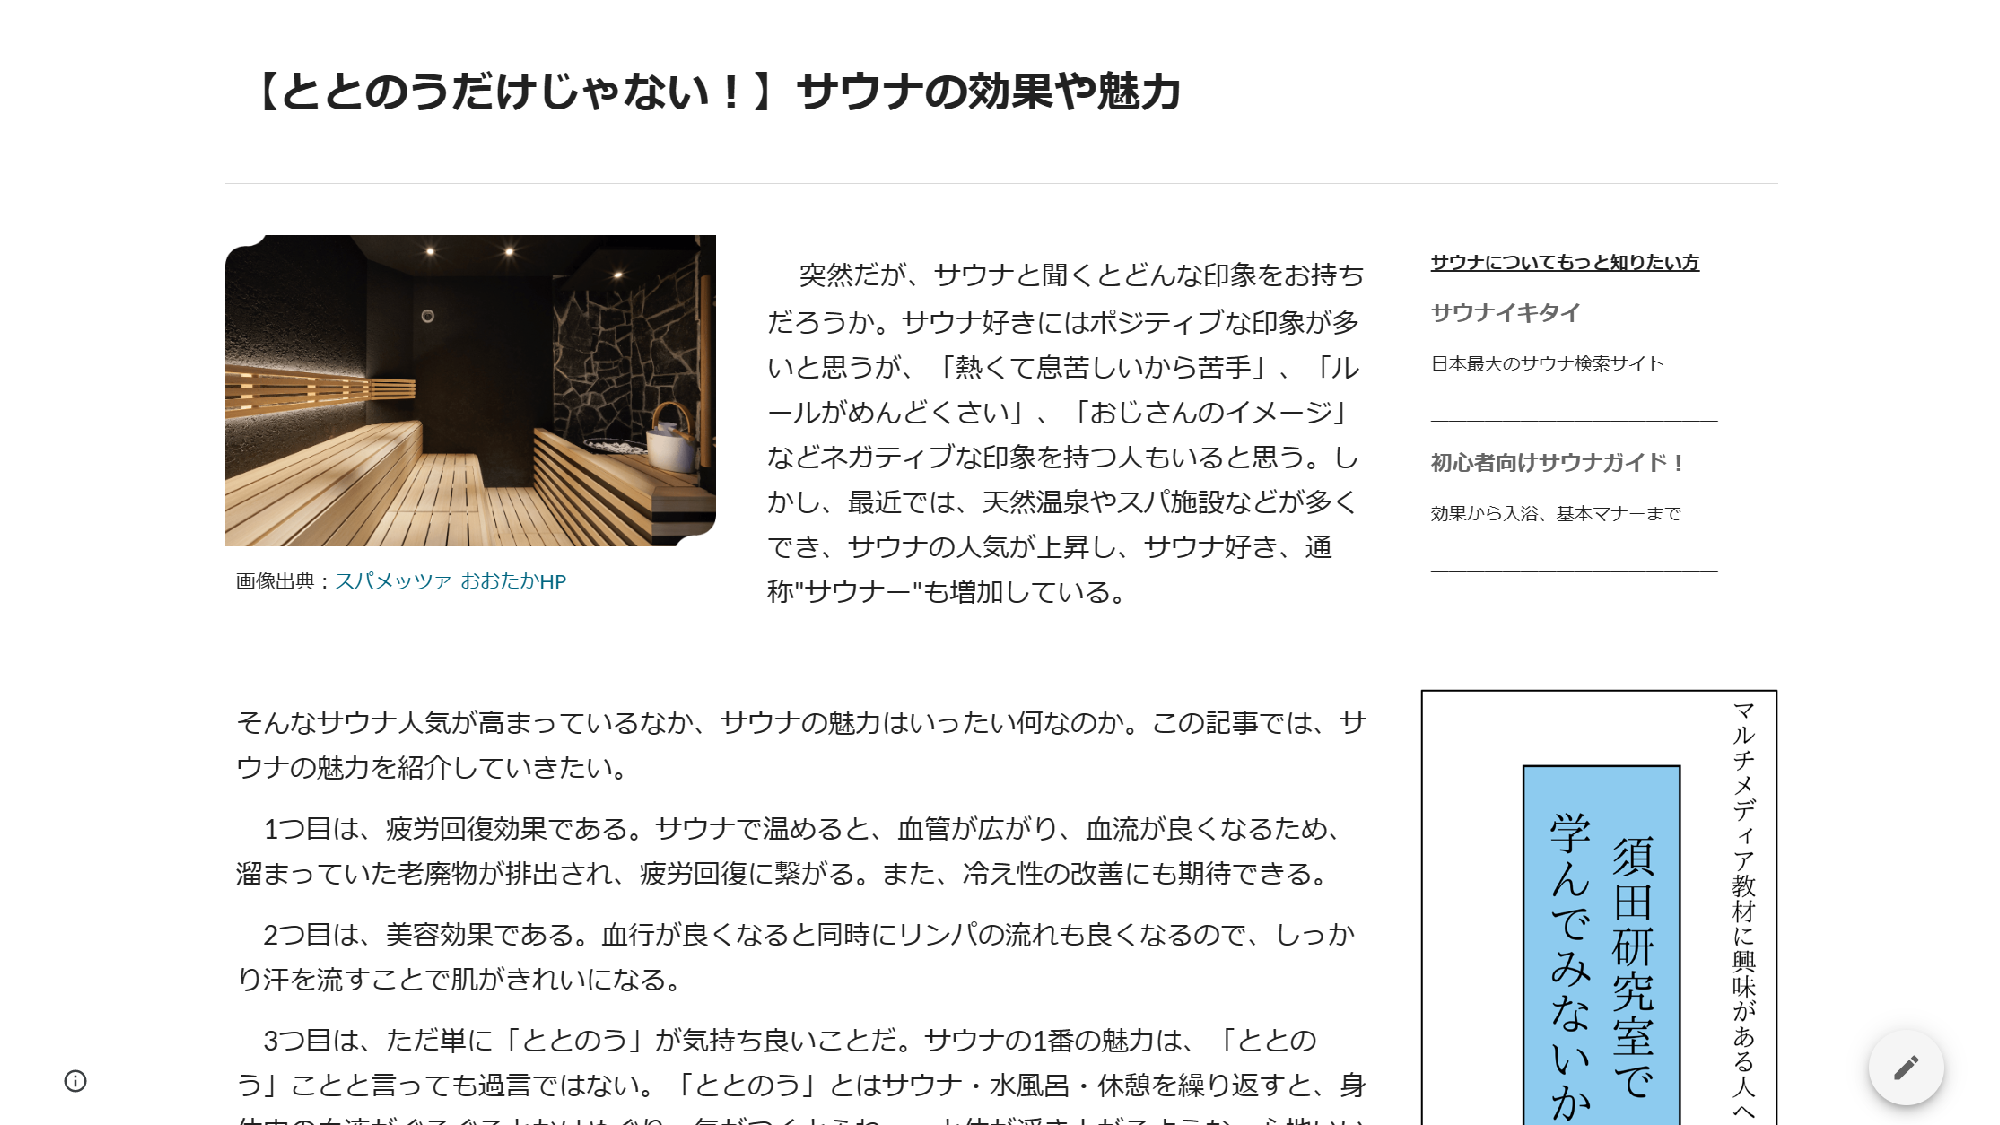
\includegraphics[height=70mm]{figures/記事右部.pdf}
\end{center}
 \caption{記事右部の配置}
 \label{fig:記事右部}
\end{figure}

\begin{figure}[H]
\begin{center}
 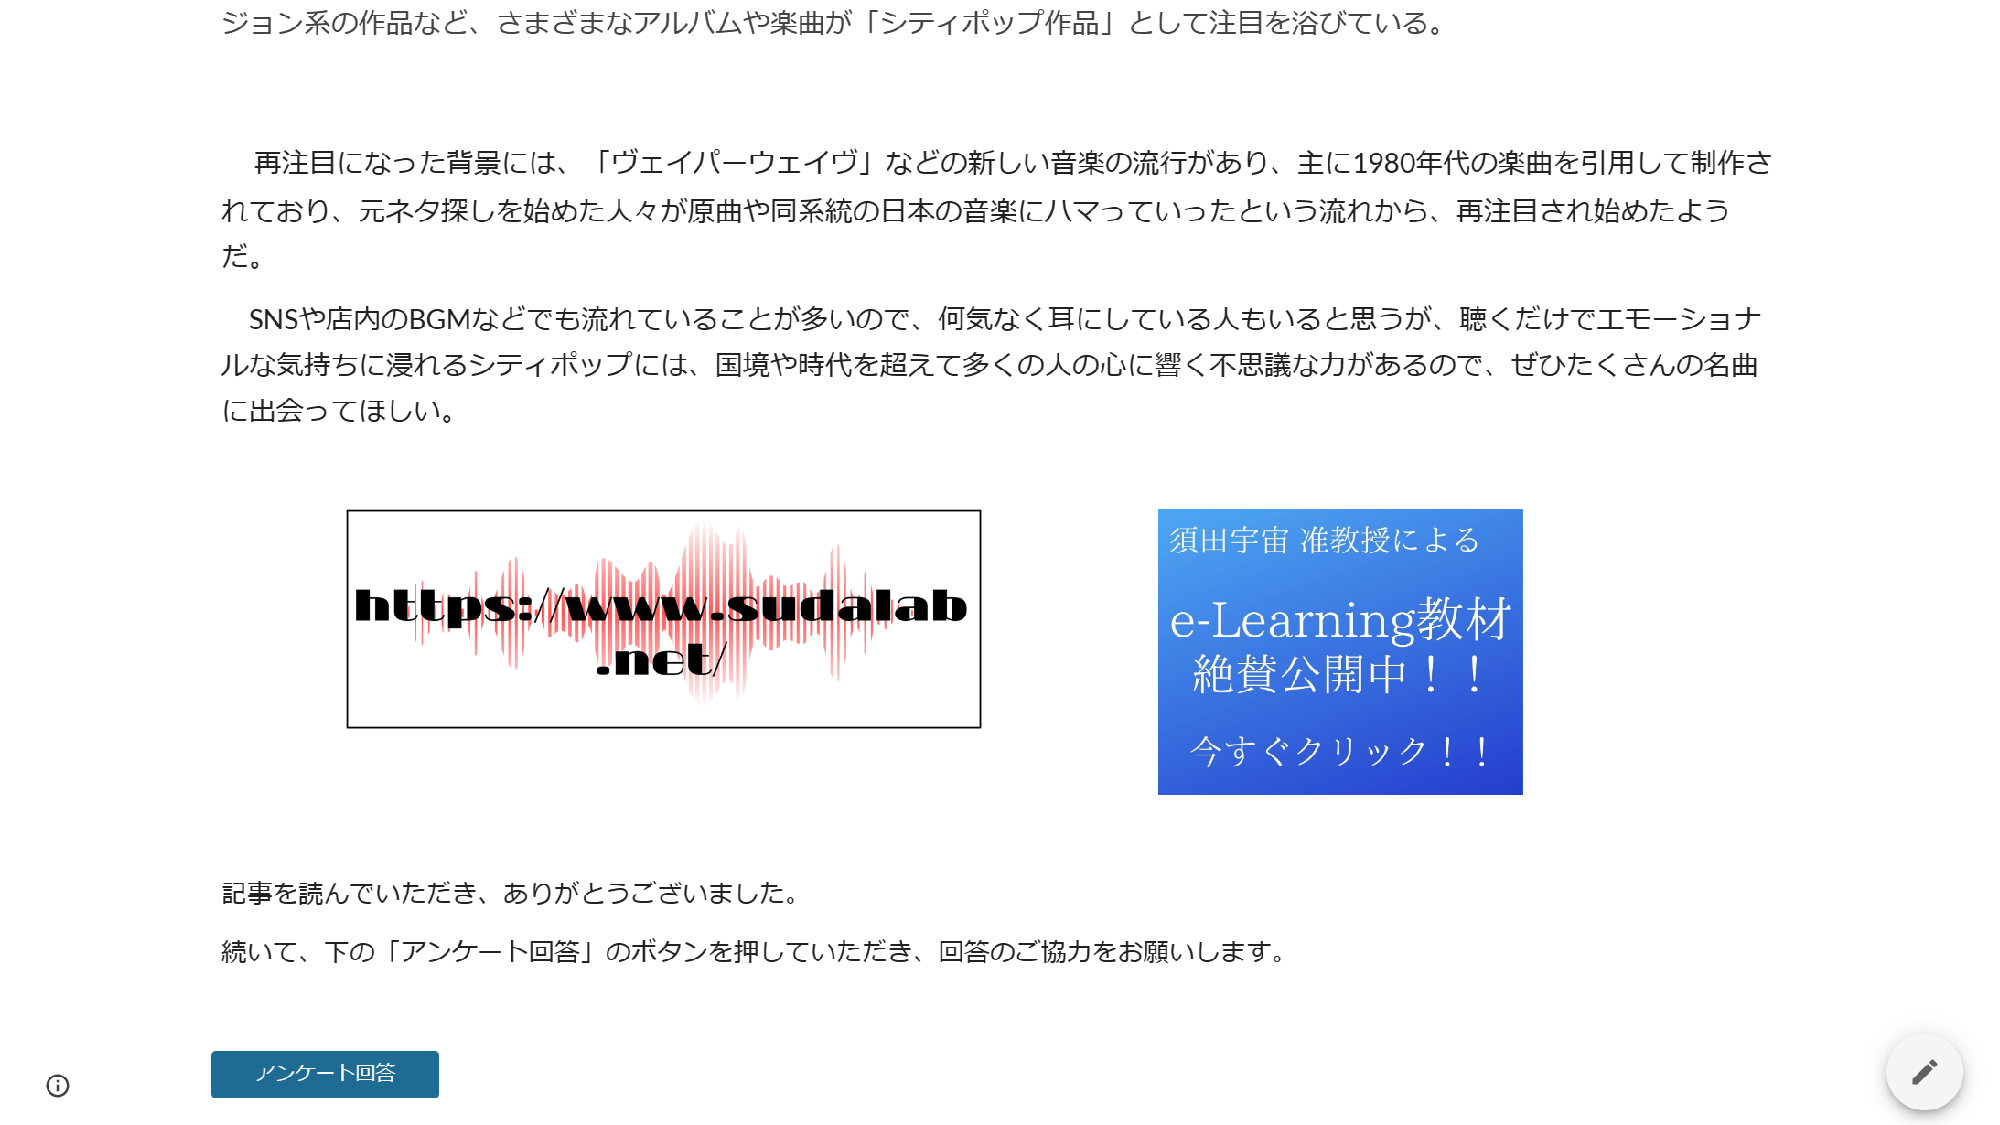
\includegraphics[height=70mm]{figures/記事終わり.pdf}
\end{center}
 \caption{記事終わりの配置}
 \label{fig:記事終わり}
\end{figure}

次に,フォントにおいては,図\ref{fig:ゴシック体}~図\ref{fig:丸ゴシック体}のようにゴシック体・明朝体・丸ゴシック体による広告を挿入している.配置においては,それぞれ差異がないように,記事右部に配置している.
フォントにおいても,主に使用されることが多いフォントであるため、この3つのパターンで比較した.

\begin{figure}[H]
\begin{center}
 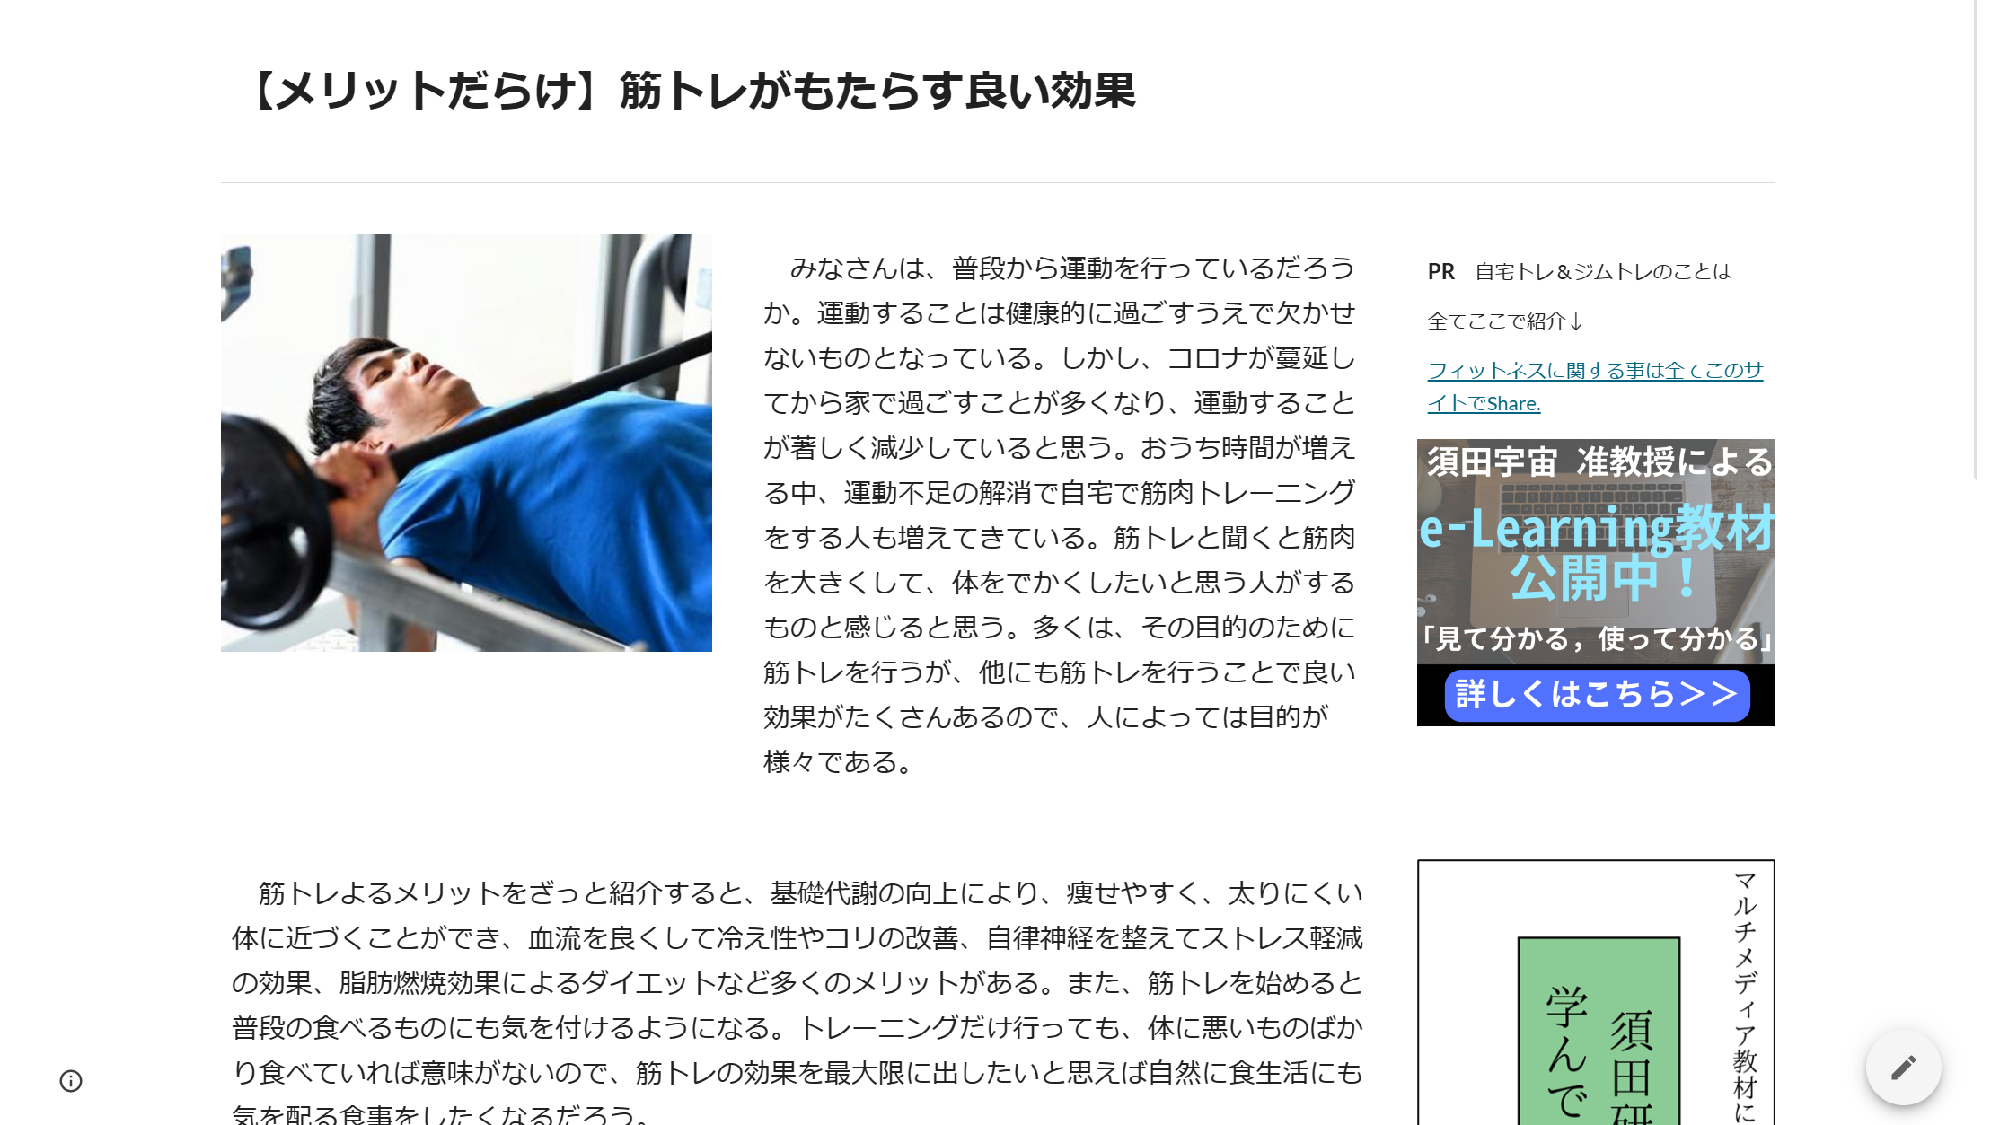
\includegraphics[height=70mm]{figures/ゴシック体.pdf}
\end{center}
 \caption{記事終わりの配置}
 \label{fig:ゴシック体}
\end{figure}

\begin{figure}[H]
\begin{center}
 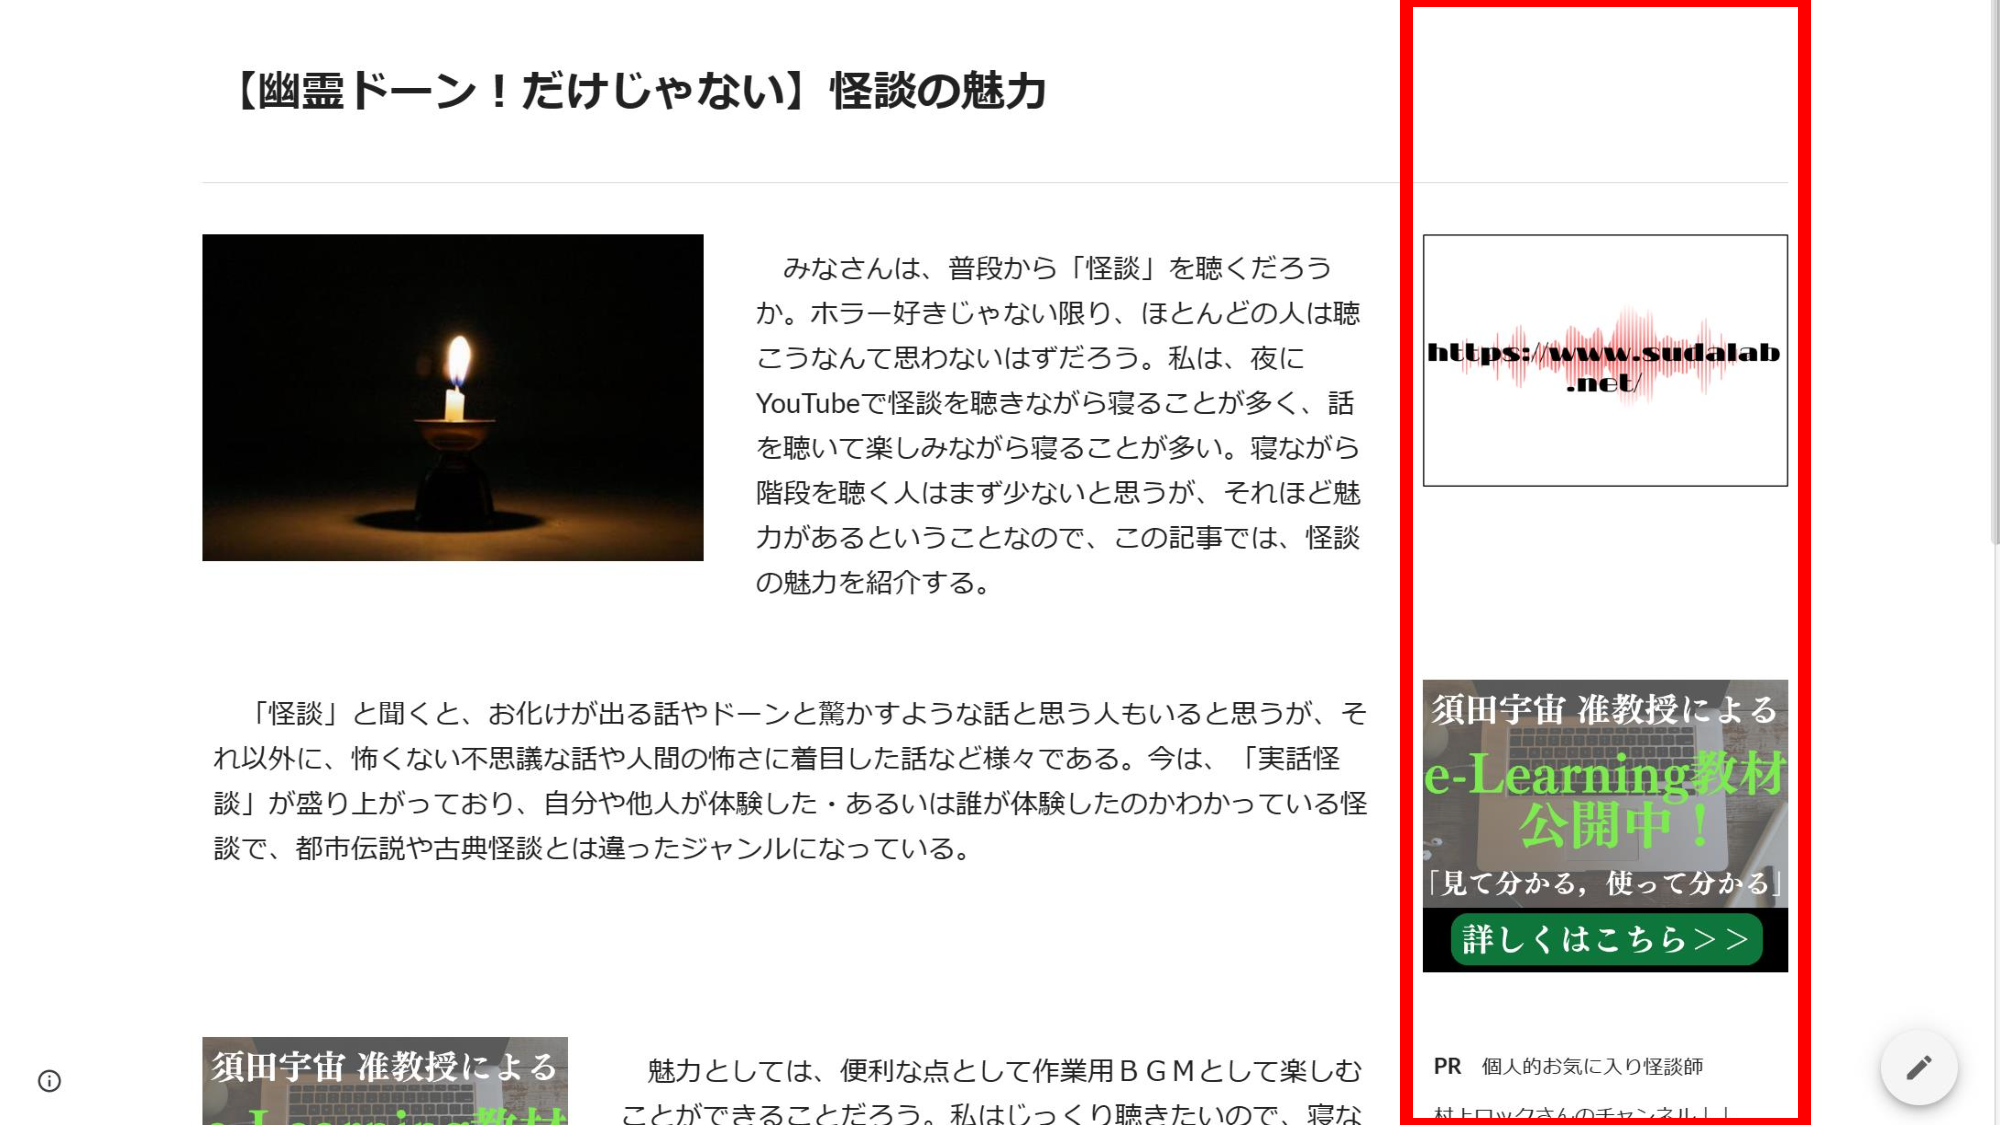
\includegraphics[height=70mm]{figures/明朝体.pdf}
\end{center}
 \caption{記事終わりの配置}
 \label{fig:明朝体}
\end{figure}

\begin{figure}[H]
\begin{center}
 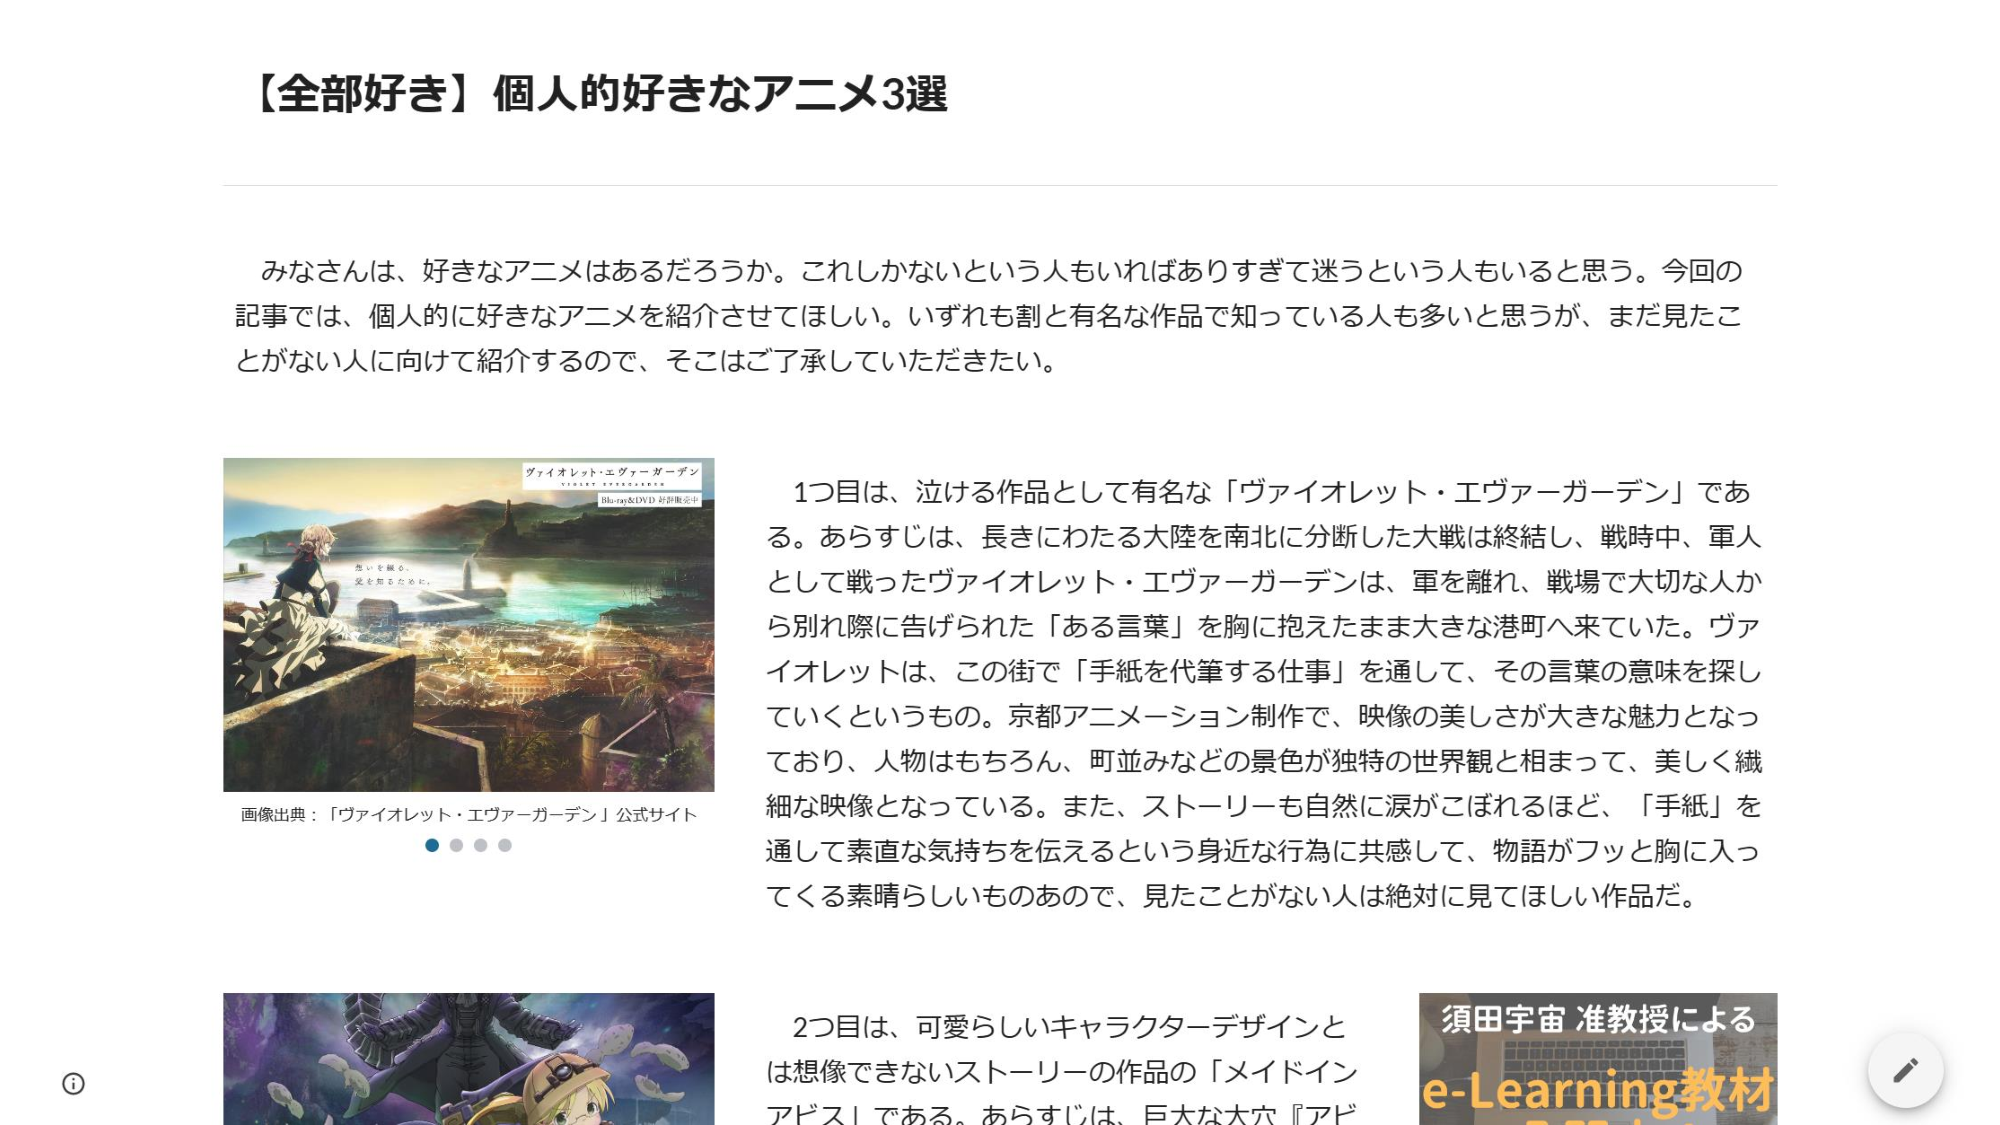
\includegraphics[height=70mm]{figures/丸ゴシック体.pdf}
\end{center}
 \caption{記事終わりの配置}
 \label{fig:丸ゴシック体}
\end{figure}

\subsection{アンケート内容}
このアンケートでは,煩わしさおよび宣伝効果に関する被験者からの評価を収集するためである.
1,2回目のアンケートの設問は共に5問で,設問内容は1回目と2回目で異なっている.
1,2回のアンケートで共通している設問としては,表示されていた広告の色やロゴ等を正しく認識できていたかというもの,どの程度煩わしく感じたかを4段階で回答してもらうもの,広告や記事に関して感じたことを書いてもらう自由記述を設けている.
1回目のアンケートでは,記事を最後まで読んでいるのかを確かめるために,記事の内容に関する設問を2問設けている.
2回目のアンケートでは,広告の印象から煩わしさや宣伝効果に関係性があるのか確かめるべく,広告に対する印象の強さを4段階で回答するもの,広告に対するイメージを6つの選択肢(格調高い・やわらかい・親しみやすい・力強い・男性的・女性的)から複数回答できるものを設けている.

\subsection{実験の流れ}
図\ref{}に,被験者から見た実験の流れを示す.
私が作成した広告が挿入されている記事のサイトを開き,最後まで読んでもらう.
次に,「アンケート回答」のボタンを押してもらい,1回目と2回目のアンケートを統合するために最初に名前を入力して,アンケートの設問に回答してもらい,上記を全て終えた被験者は実験完了となる.

\clearpage

\section{結果}
\subsection{1回目のアンケート}
図\ref{fig:広告認識正答率_1}に配置方法による各広告の認識正答率を示す.
記事内は73.7\%,記事右部は65.8\%,記事終わりは76.3\%となり,広告の認識率が高いのは,記事終わりとなった.
また,それぞれのパターンの記事のアンケートを答えてくれた人数が違うので,3つの記事のアンケートを全て答えた人数に合わせたため,38人となった.

\begin{figure}[h]
\begin{center}
 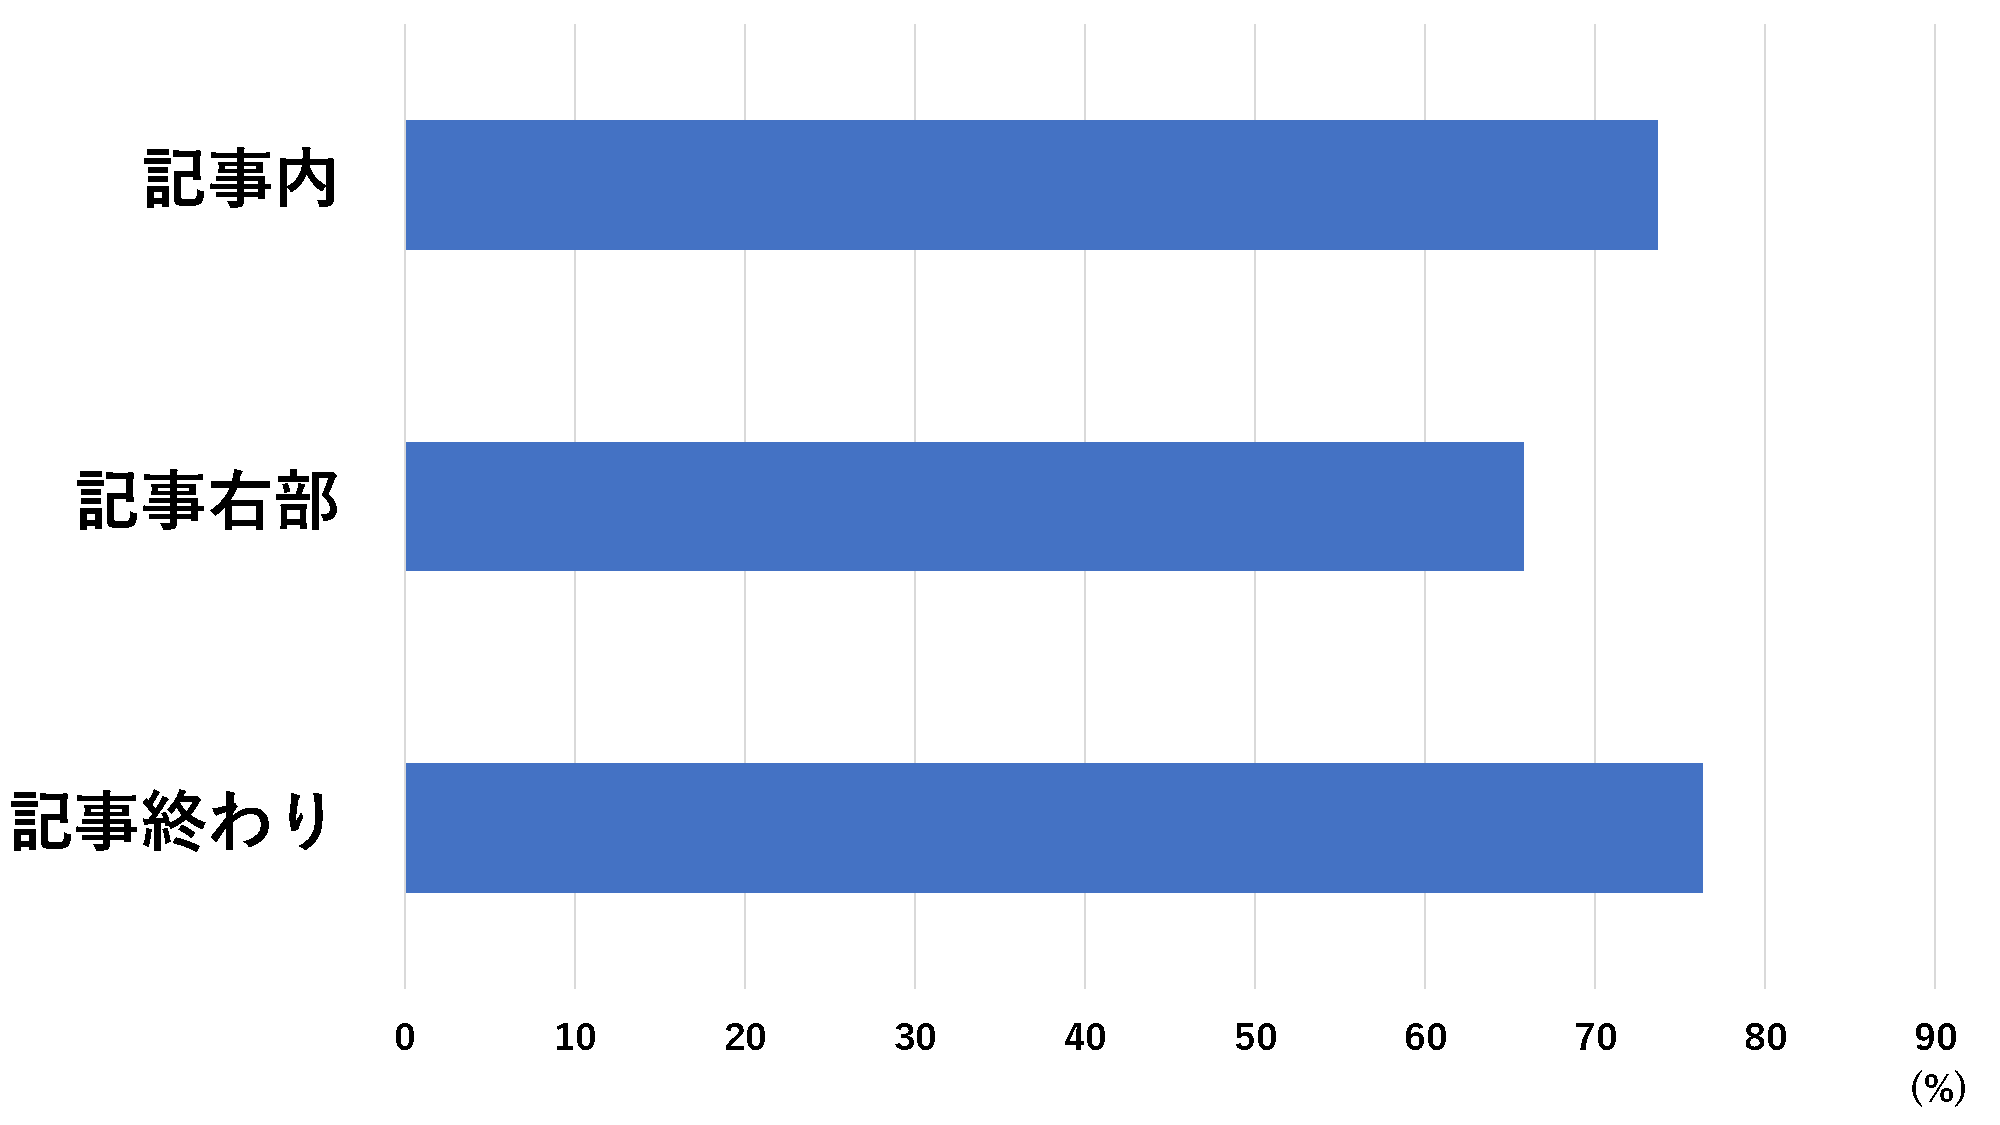
\includegraphics[height=65mm]{figures/広告認識正答率_1.pdf}
\end{center}
 \caption{1回目のアンケートの認識正答率}
 \label{fig:広告認識正答率_1}
\end{figure}

次に,図\ref{fig:煩わしさ_1}に各広告配置方法について被験者が評価した煩わしさを,評価した被験者の人数で示す.
各配置とも,半数以上が「煩わしくない」もしくは「あまり煩わしくない」と回答しており,記事内が他の配置よりも「少し煩わしい」と回答する人が多かった.

\begin{figure}[h]
\begin{center}
 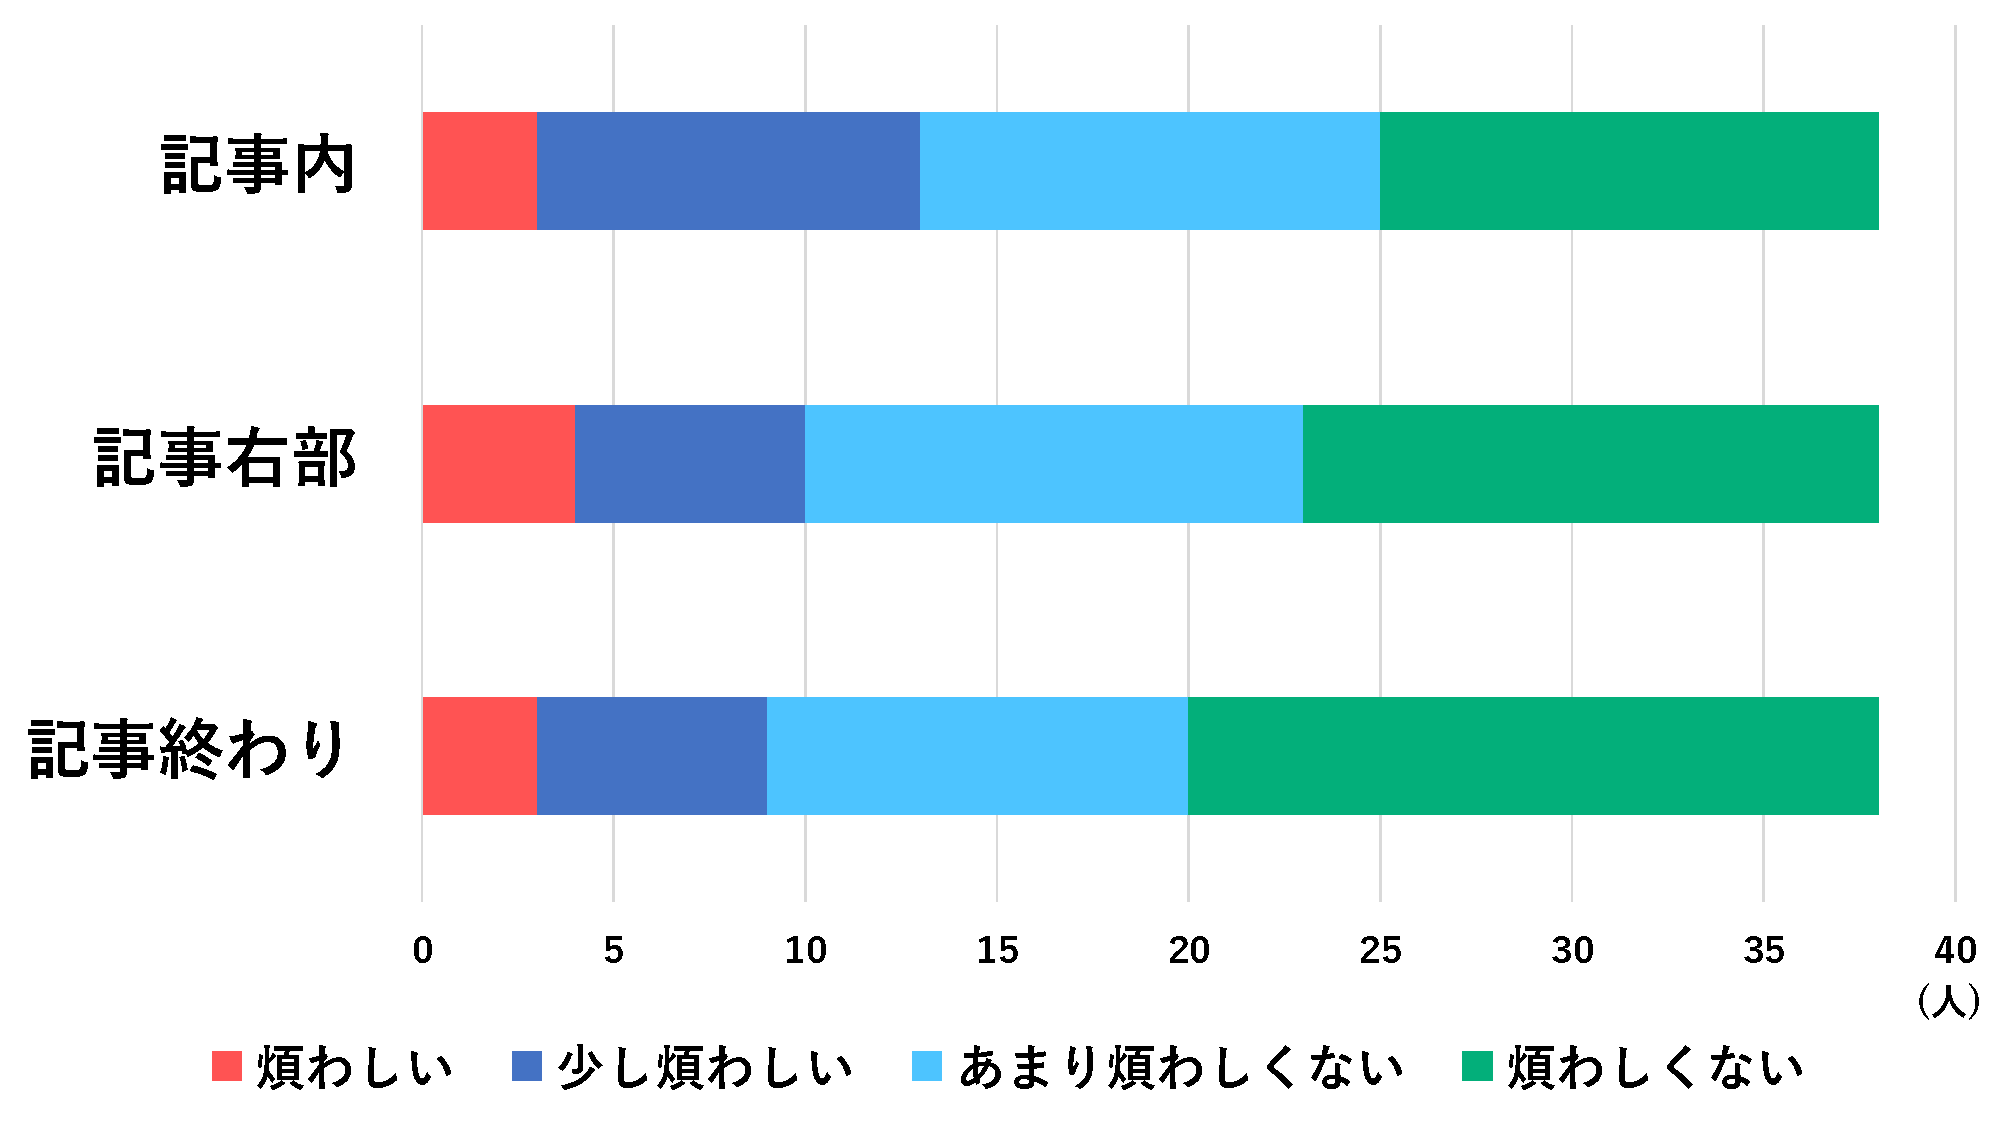
\includegraphics[height=65mm]{figures/煩わしさ_1.pdf}
\end{center}
 \caption{各配置の煩わしさの程度の4段階評価}
 \label{fig:煩わしさ_1}
\end{figure}

\subsection{2回目のアンケート}
図\ref{fig:広告認識正答率_2}にフォントによる各広告の認識正答率を示す.
ゴシック体は62.9\%,明朝体は74.1\%,丸ゴシック体は84.6\%となり,広告の認識率が高いのは,丸ゴシック体となった.
また,1回目と同様,それぞれのパターンの記事のアンケートを答えてくれた人数が違うので,3つの記事のアンケートを全て答えた人数に合わせたため,26人となった.

\begin{figure}[h]
\begin{center}
 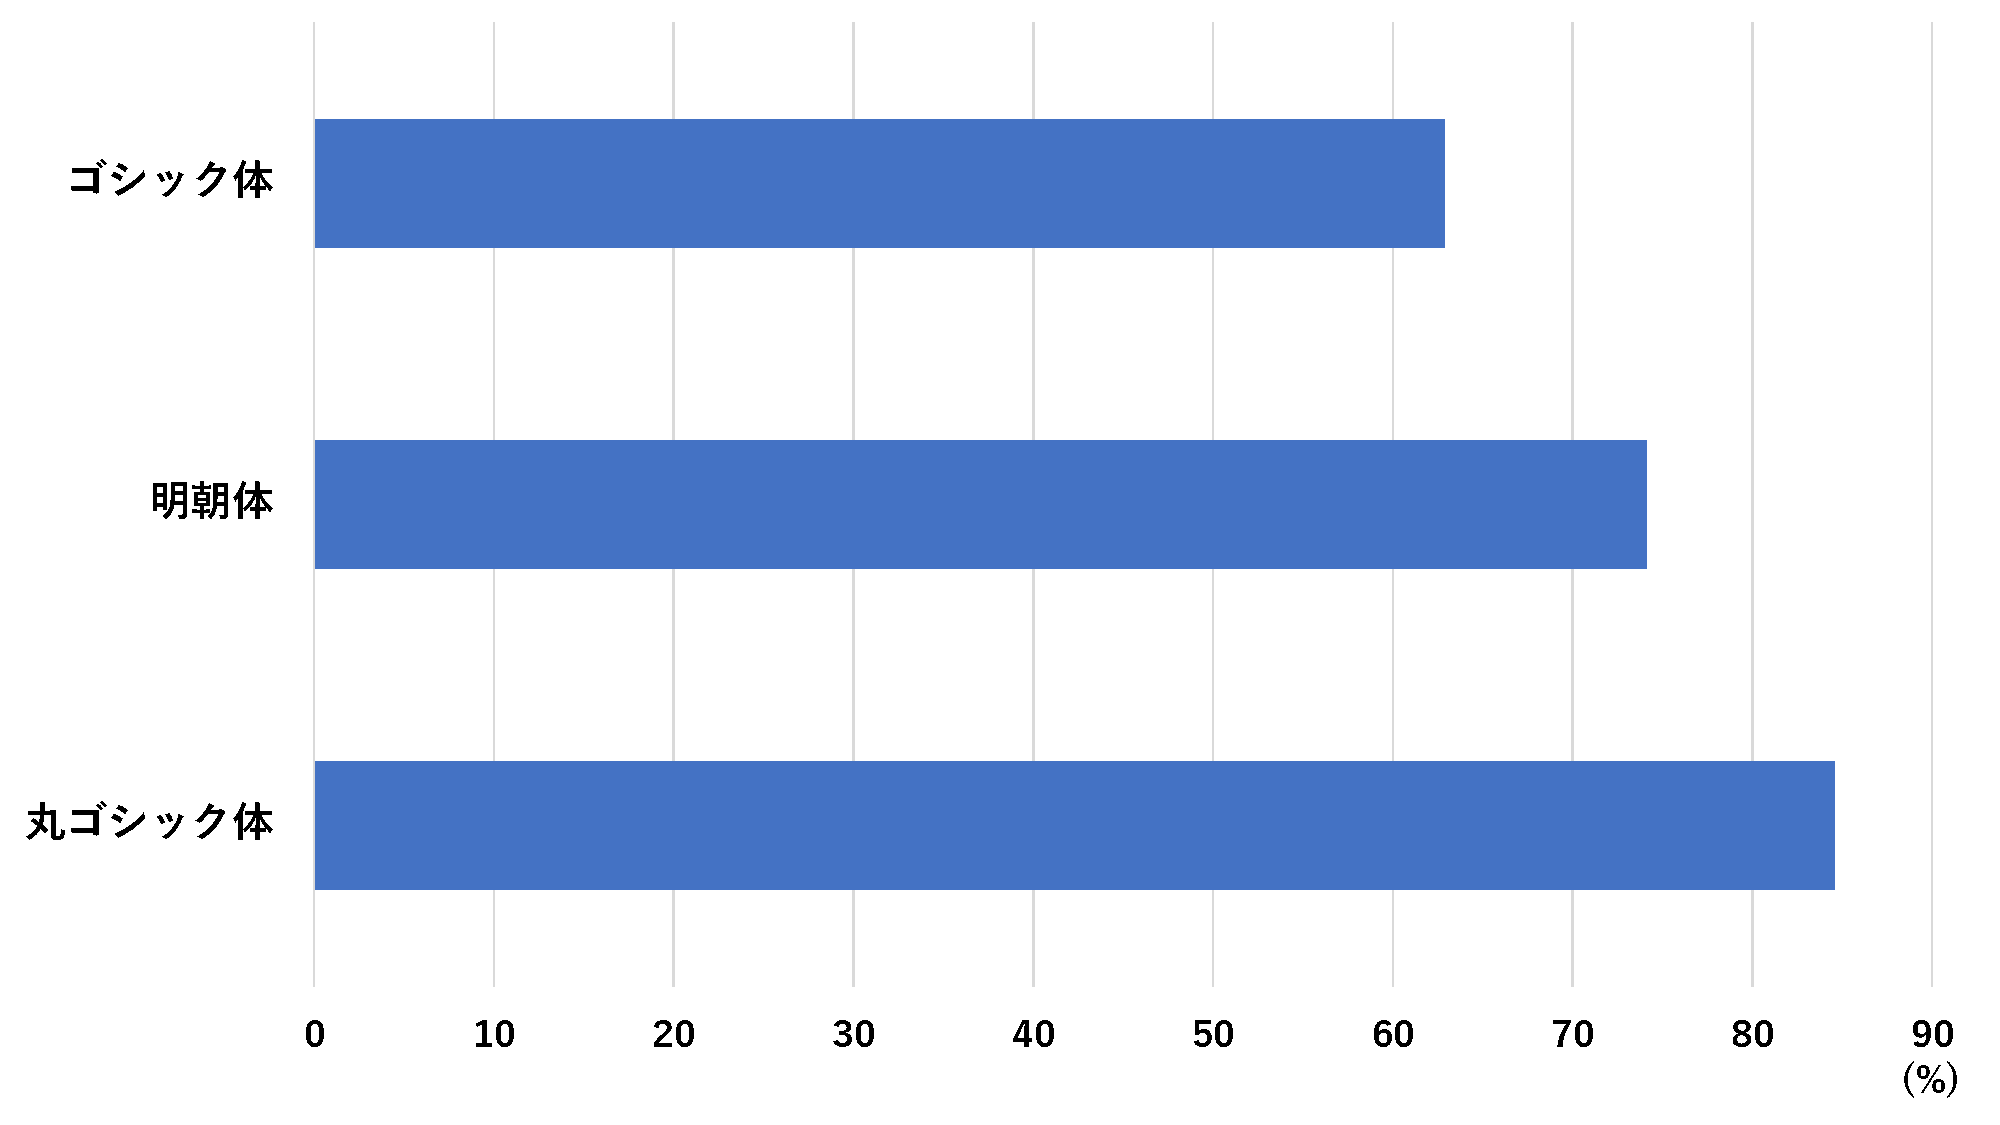
\includegraphics[height=65mm]{figures/広告認識正答率_2.pdf}
\end{center}
 \caption{2回目のアンケートの認識正答率}
 \label{fig:広告認識正答率_2}
\end{figure}

次に,図\ref{fig:煩わしさ_2}に各フォントについて被験者が評価した煩わしさを,評価した被験者の人数で示す.
1回目同様,各フォントとも,半数以上が「煩わしくない」もしくは「あまり煩わしくない」と回答しており,明朝体が他のフォントよりも「少し煩わしい」,「煩わしい」と回答する人が多かった.

\begin{figure}[h]
\begin{center}
 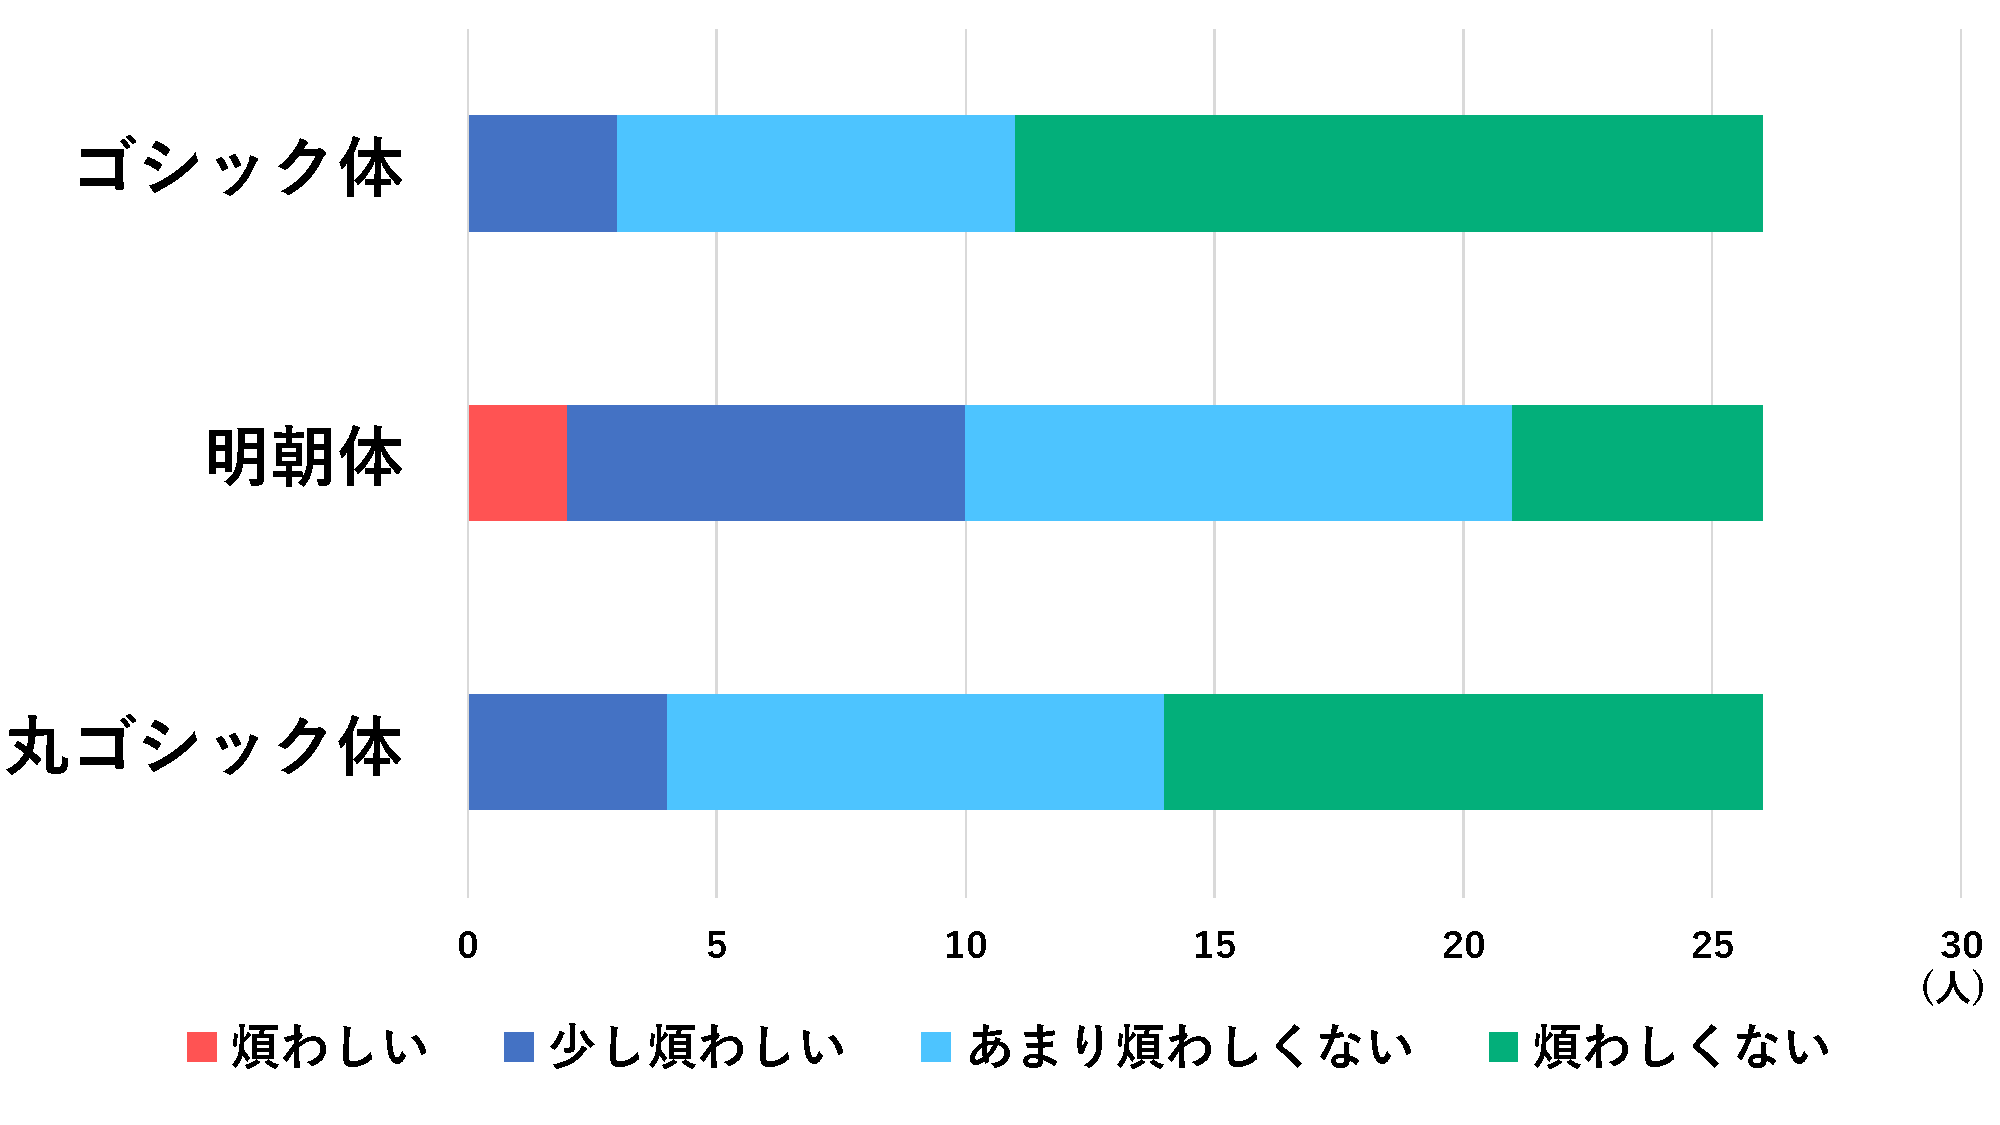
\includegraphics[height=65mm]{figures/煩わしさ_2.pdf}
\end{center}
 \caption{各フォントの煩わしさの程度の4段階評価}
 \label{fig:煩わしさ_2}
\end{figure}

\clearpage

\section{考察}

\clearpage

\section{結言}

\clearpage

\section{謝辞}
本研究の遂行及び本論文の作成にあたり,多大なる御指導,御助言を頂きました須田研究室の仲間に深く感謝の意を表します.
そして,何よりも本論文の作成にあたり,多大なる御指導,御助言をいただきました,須田 宇宙准教授に深く感謝の意を表します.

\clearpage

\begin{thebibliography}{99}
\bibitem{mobile} 中島 弘貴,柗本 真佑,楠本 真二, ``モバイル端末におけるWeb広告の配置方法に対する一検討'', 信学技報, vol.117, no.389, LOIS2017-62, pp.69-74, 2018年
\bibitem{dentsu} 株式会社電通, ``2021年 日本の広告費'', \url{https://www.dentsu.co.jp/news/release/2022/0224-010496.html}, 2022/7/29参照
\end{thebibliography}

\end{document}